\documentclass{standalone}

\usepackage{amsmath,amsfonts,amssymb,amsthm,mathtools} 
\usepackage{fontspec}            % пакет для подгрузки шрифтов
\setmainfont{Burst My Bubble}   % задаёт основной шрифт документа

% why do we need \newfontfamily:
% http://tex.stackexchange.com/questions/91507/
\newfontfamily{\cyrillicfonttt}{Burst My Bubble}
\newfontfamily{\cyrillicfont}{Burst My Bubble}
\newfontfamily{\cyrillicfontsf}{Burst My Bubble}
% Иногда тех не видит структуры шрифтов. Эти трое бравых парней спасают ситуацию и доопределяют те куски, которые Тех не увидел.

\usepackage{unicode-math}     % пакет для установки математического шрифта
\setmathfont{Asana Math}      % шрифт для математики

\usepackage{polyglossia}      % Пакет, который позволяет подгружать русские буквы
\setdefaultlanguage{russian}  % Основной язык документа
\setotherlanguage{english}    % Второстепенный язык документа

\usepackage{pgf,tikz,pgfplots}
\usetikzlibrary{arrows,calc}
\usepackage{relsize} 

\usepackage{graphicx} 
\usepackage{rotating}
\usepackage{xcolor}
\usepackage{color}

%\newcommand{\Big}{\fontsize{50}{60}\selectfont Foo}

\definecolor{bl}{HTML}{333333}
\definecolor{darkbl}{HTML}{1000A5}


\begin{document}

\centering

\begin{tikzpicture}[scale=2]
\begin{scope}[rotate=30]  
% Radius of regular polygons
  \newdimen\R
  \R=2cm
  \coordinate (center) at (0,0);
 \draw (0:\R)
     \foreach \x in {60,120,...,360} {  -- (\x:\R) }
              -- cycle (300:\R)
              -- cycle (240:\R)
              -- cycle (180:\R)
              -- cycle (120:\R)
              -- cycle (60:\R)
              -- cycle (0:\R)  [line width=1.9mm,color=bl,fill=white,fill opacity=0.1];
\end{scope}
       
% picture with sex
    \node[inner sep=0pt] (russell) at (0,0)
    {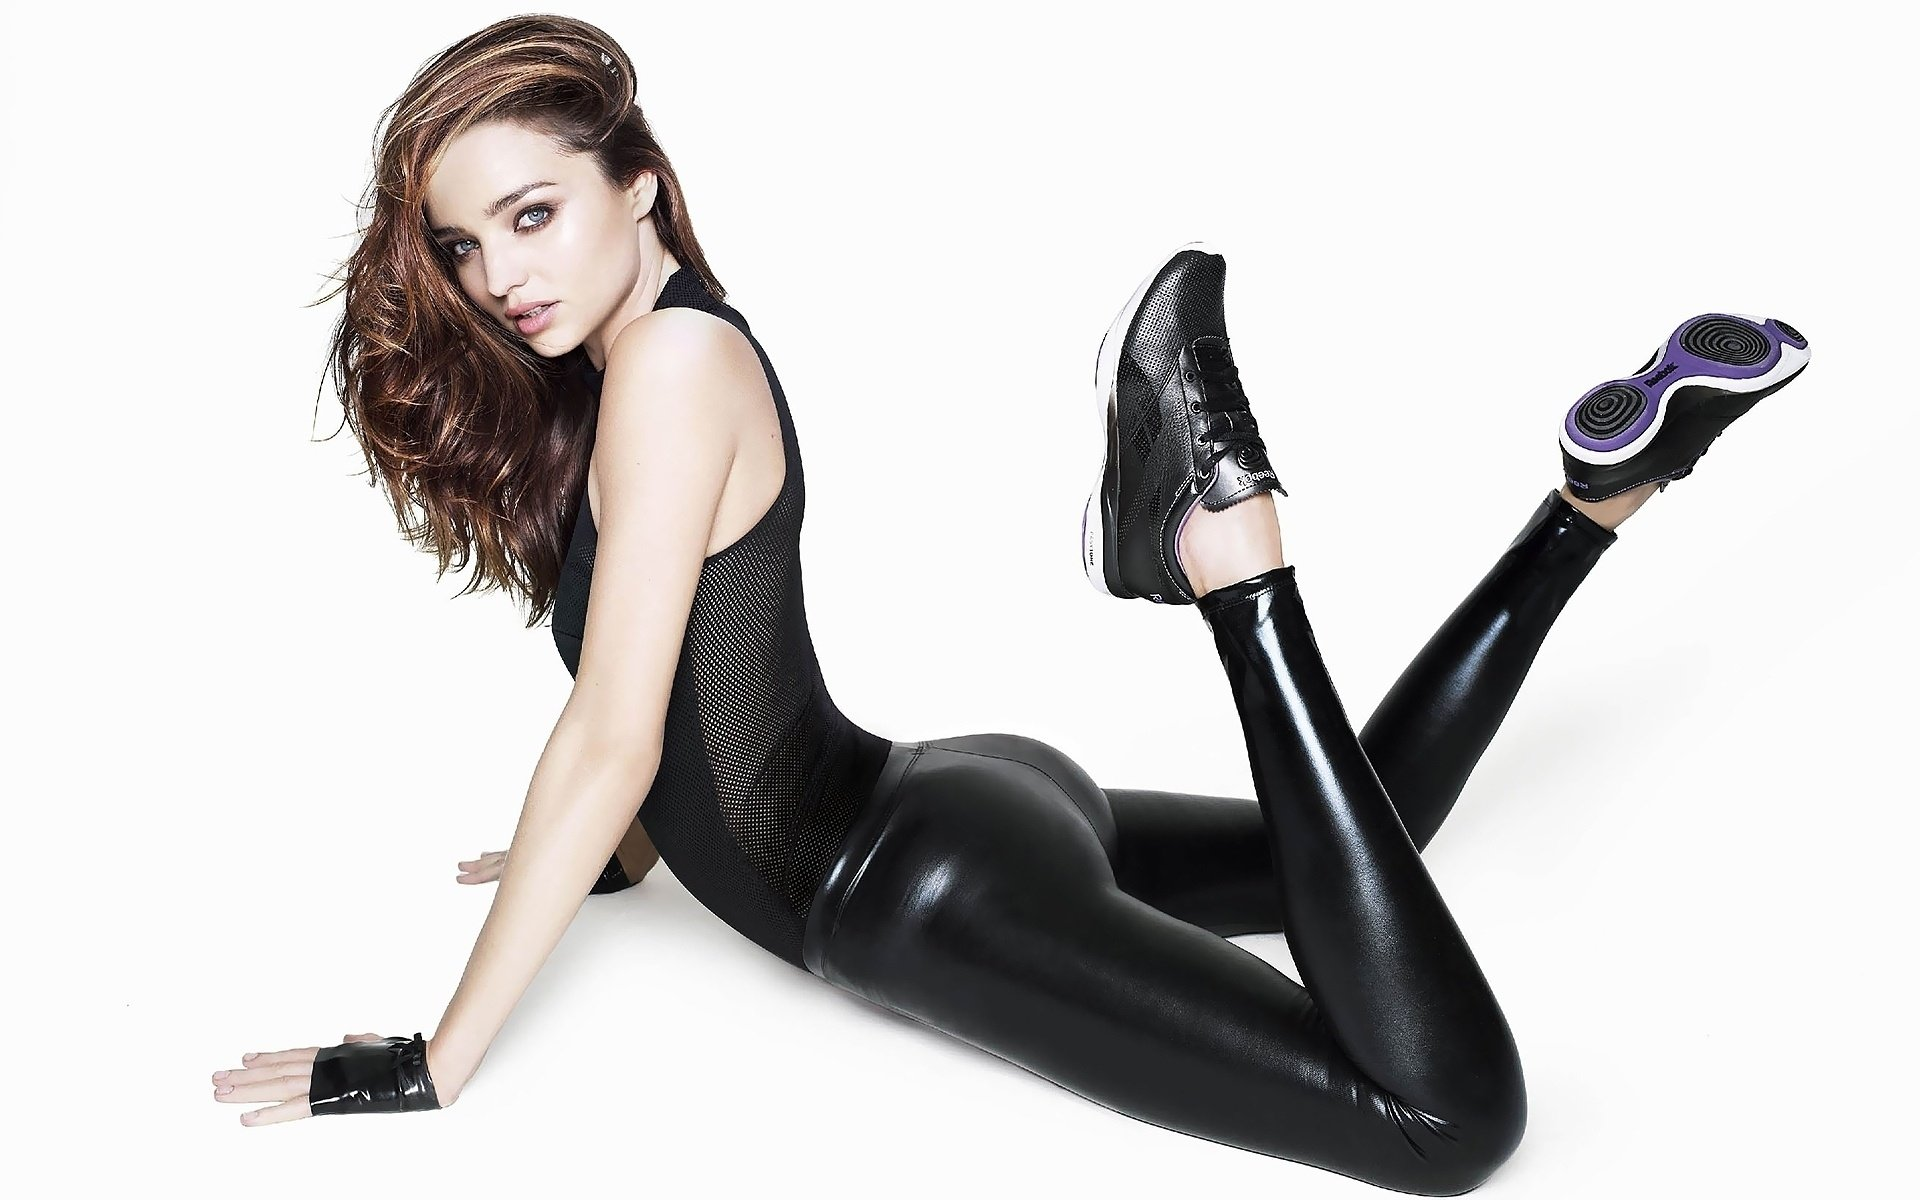
\includegraphics[angle=0,scale=0.08]{sex.jpg}};               

% caption 
\draw[color=black,draw,align=left] (-0.9,1.2) node[right] {\Huge \textbf{MMMMMMM......}};             
\draw[color=black,draw,align=left] (-0.68,-1.3) node[right] {{\fontsize{30}{60}\selectfont \fontspec{Amiri}{\LaTeX...}}};                   
\end{tikzpicture}

\end{document}
